% !TeX root = ../main.tex
% Add the above to each chapter to make compiling the PDF easier in some editors.

\chapter{Methods}\label{chapter:methods}

\section{Dataset}
Datasets such as CAMS \parencite{CAMS} or TNO \parencite{TNO_LowRes}  provide GHG emissions in a 0.1 times 0.05 lat times long resolution which corresponds to ~5 by ~5 kilometers.
This resolution is very low and urban data cannot effectively be extracted.
For instance, a city contained within a 30km by 30km grid, would contain 6 by 6 cells.
This is not enough to draw any meaningful information and conclusion. 
Therefore, this thesis focues on the high res $2015$ \parencite{TNO_HighRes15} and $2018$ \parencite{TNO_HighRes18} TNO datasets are used.
These are two high resolution, roughly 1km by 1km, emission inventory and thus high resolution emission fields in urban environments can be extracted.
The inventory contains GHG emissions for each GNFR sector \parencite{GNFR_Sectors}, with the road sector $F$ being split into $4$ sub sectors, for each coordinate in a defined grid within Europe.
This results in $15$ emission values per gas per cell.
For this thesis, only CO2 from fossil fuels are considered.
However, the presented approaches can be directly applied for all types of GHG sources.

\subsection{Urban Emission Fields}
Urban environments differ from non-urban environments in terms of their emissions.
For instance, urban environments often have a city center that generates a large portion of emissions as seen for example in Munich (Figure).
Therefore, as the focus of this thesis are urban environments, they have to be filtered from the TNO datasets.
For this, a number of cities are selected from a public database by OpenDatasoft \parencite{OpenDataSoft}.
Cities are filtered according to their population size.
For this thesis, the population threshold is set to $100.000$.

From the filtered cities, the coordinates are used to extract emission fields.
From the TNO dataset, $51$ by $51$ grids around the city center are extracted.
This corresponds to a dimension of n km by n km.
While most cities are not even close to this size, this allows to later crop the fields to a desired size.
For this thesis, emission fields have $32$ by $32$.

Some cities may be too close to each other and thus result in leakage of data to test and validation sets.
Thus, cities are filtered if they are too close to other cities.
The following algorithm is used to guarantee no overlapping data.
1) Get all cities currently extracted and determine the lat and lon distances to the current city
2) Determine all cities that are within a threshold
3) If there are none, add the current city and proceed to next city
4) Else, check if the current city has a greater population size that all other cities that overlap
5) If yes, removed the overlaping cities and add the current city to the cities.
6) Else, ignore the city and proceed with next city

The overall resulting amount of citiy emission fields per year, $2015$ and $2018$, is then $106$.
A list of all cities with the corresponding coordinates is appended in the appendix.

The number of extracted emission fields is not enough to train a generative model.
Thus, temporal scaling factors from (cite) are used to generate more samples.
Scaling factors are applied to individual GNFR sectors.
This results in $24 * 7 * 12 = 2016$ samples per city per year.
The resulting combined dataset size is thus $106 * 2 * 2016 = 45792$ individual emission fields with size $51$ by $51$.
To reduce the memory overhead, scaling factors are applied at sampling time and only the original data is kept in memory.

\subsection{Dataset Filtering}
% The dataset contains many cities.
% However, not all of these cities have comparable emission fields.
% In other terms, there may be outliers contained in the dataset that can throw of the trianing and evaluation of the model.
% Especially since there are not many cities, outliers harm the training and evaluation of the model significantly.
T.b.d.

\subsection{Dataset Split}
The emission fields are split into training, validation, and test data.
The test data is used for experiments and evaluations and makes up $t$ percent of the data.
The model does not see the test data during training.
The validation data is used to evaluate the generalization capabilities of the model during training and makes up $v$ percent of data.
Finally, the training data is used to train the model and updates its weights and makes up $1 - v - t$ of the data.

To split the data deterministically and reproducibly, the city names are sorted alphabetically.
Then, the first $t$ percent of city names are assigned to the test set.
Of the remaining $1 - t$ percent of city names, the first $\frac{v}{1 - t}$ percent are assigned to the validation set.
The remaining city names are assigned to the training data.

Maybe make a diagram here.

\subsection{Data Augmentation}
To improve the generalization abilities of the model CITE, common image augmentation techniques are applied (to cite) to the emission fields in the training data.
First, random cropping is used.
Furthermore, a random horizontal flip and vertical flip are applied with probability $0.5$ each.
Lastly, emission fields are randomly rotated by 90$\circ$ with probability of $0.5$.
This results in $8$ different transformations, with one of them being the original emission field.

The validation and test emission fields are not transformed, except for a center crop.

\subsection{Scaling}
Scaling is an important factor for machine learning.
Large-scale data can make training converge slow and instable (cite).
Furthermore, regularization techniques such as batch normalization rely on scaled values (cite).
A common technique for scaling values is min max scaling (cite).
However, min max scaling is sensitive to outliers and thus not ideal for emission inventories where range of emissions within a city can largely differ.
Instead, robust scaling (cite) can be applied.
To determine a good scaling factor, the $95$th percentile of values is determined for each city in the training set.
The inverse of the average is then used as the scaling factor.
The resulting scaling factor is thus $\frac{1 a}{2.5 * 10^6 kg}$

\section{Variational Autoencoder}
Some text about generative models and variational autoencoder (cite) in its original form being the chosen one.

\subsection{Architecture Search}
Searching for optimal hyperparamaters is a challenging task with many different approaches (cite).
In particular, designing a good architecture takes a lot of trial and error.
Thus, different architectures are explored to determine a suitable one.
For this, first a basline architecture is established.
Then, different variations of this architecture are explored and trained.
The architecture of the model with the best performance is then chosen as the model architecture for this thesis.

Each variation is trained with for $20$ epochs on the TNO 2015 data only to decrease the architecture bias during search.
The dataset split is $t=0.15$, $v=0.15$, with the test set not being used at all.
The batch size is $32$.
As optimizer AmsGrad is used (cite) with a learning rate of $1$.
Gradients are clipped at $0.5$.
% Add any further hyperparameters.

\subsection{Baseline Architecture}
The baseline architecture is inspired by (Walking the Tightrope: An Investigation of the Convolutional Autoencoder Bottleneck cite).
This means that the bottleneckl layers have a high width and height.
As the input width and height of the emission fields are $32$ by $32$, the Bottleneck width and height are chosen as $8$ by $8$.
Inspired by "Striving for Simplicity: The All Convolutional Net" (cite), to reduce the width and height dimensions, instead of using pooling operations, $2$ strided convolutions are used.
The strided convolutions, depicted in Figure, have kernel 2 and stride 2, thus halfing the size.
\begin{figure}[h!]
    \centering
    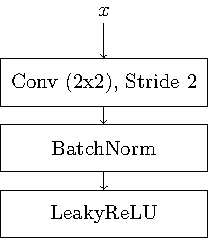
\includegraphics[]{figures/model_architecture/build/conv_layer.pdf}
    \caption{Conv Layer}
\end{figure}
The strided convolution layers make use of the LeakyReLu activation function (cite) and batch normalization (cite), as a regularization technique.

Vice versa, in the decoder, 2 strided transpose convolutions with the same parameters are used to double the width and height.
\begin{figure}[h!]
    \centering
    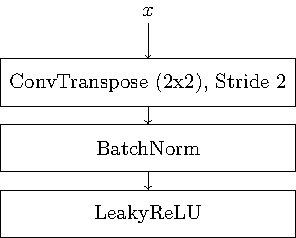
\includegraphics[]{figures/model_architecture/build/deconv_layer.pdf}
    \caption{DeConv Layer}
\end{figure}

In between the strided convolutions residual convolutional layers (ResConv) (cite) are used.
They can be seen in Figure.
\begin{figure}[h!]
    \centering
    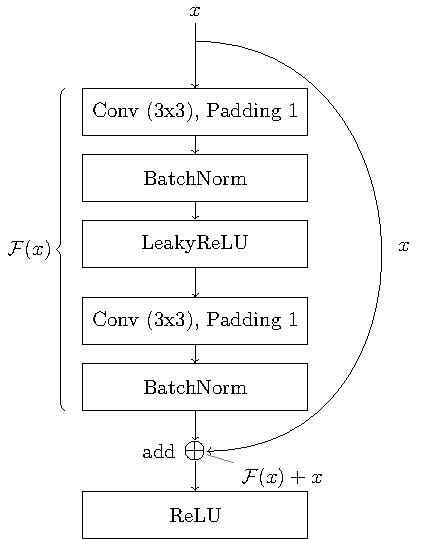
\includegraphics[]{figures/model_architecture/build/residual_conv_layer.pdf}
    \caption{ResConv Layer}
\end{figure}
The ResConv layers make use of two convolutions with kernel 3 and padding 1 to retain the width and height dimensions.
The output activation is ReLu (cite).
In between the two convolutional layers, LeakyReLu is used again.
Again, batchnorm is applied.
\begin{figure}[h!]
    \centering
    \includegraphics[width=\textwidth]{figures/model_architecture/build/vae_encoder.pdf}
    \caption{Baseline Encoder Architectur (generated with (https://github.com/HarisIqbal88/PlotNeuralNet?tab=readme-ov-file) (cite))}
\end{figure}
\begin{figure}[h!]
    \centering
    \includegraphics[width=\textwidth]{figures/model_architecture/build/vae_decoder.pdf}
    \caption{Baseline Decoder Architecture}
\end{figure}
As can be seen in Figure and Figure, the 2 strided convolutions are located between $2$ layers of ResConv layers each, in the encoder and decoder.
Fully connected layers are used at the end of the encoder and beginning of the decoder to achive a hidden dimension $256$ of the latent space. 
The number of parameters is \dots.

The loss function used is the typical VAE loss with MSE loss and \dots .
\begin{equation}
    L(x, \hat{x}) = 1 + 2
\end{equation}
In addition to the loss, at each step the SSIM (cite) is computed as it provides qualitatively better comparison between two emission fields than the MSE as it takes structure into account.

\subsection{Explored Variations}
The following variations are explored
\begin{enumerate}
    \item conv layers to increase / decrease depth and pooling layers to decrease width/height and upsample layers to increase width/height
    \item 3 layers everywhere
    \item residual layers based on "Identity Mappings in Deep Residual Networks" (cite) instead of ResConv layers from Figure
    \item dropout (cite) (look at "Wide Residual Networks" for source for Dropout) based on "Wide Residual Networks" (cite)
\end{enumerate}

\subsection{Final Architecture}
The final model is trained on both the TNO 2015 and 2018 data.
\dots

\section{Evaluation}

\subsection{Gaussian Measurements}
In order to evaluate the generative capbailities in the context of inverse problems, a compressed sensing problem is used for evaluation.
This compressed sensing problem is based on the paper by Bora et al. as they mention that the performance of generative models can be assesed based on their provided problem statement.
For this, a identically independent distributed matrix $A \in R^{m \times 15000}$ is sampled for each run.
The following inverse problem is then solved using the minimization problem proposed by Bora et al.
\begin{equation}
    y = A x + \epsilon
\end{equation}
with $x$ being the emission fields $x^*$ in vectorized form.
This inverse problem is equivalnt to taking taking $m$ measurements that is randomly linearly affected by any sector in any cell within the emission field grid.
While this does not correspond to a typical transport model which follows the law of physics, this problem serves as a good proxy for evaluating the generative capbailities in the context of inverse problems of the trained VAE. 

The evaluation is performed on scaled emission fields.

The resulting pipeline is the following:
\begin{enumerate}
    \item Generate random A
    \item Sample x from test set
    \item Vectorize x
    \item Compute y from forward model
    \item Run reconstruction algorithm (minimization problem)
    \item Unvectorize resulting x dach
    \item Compare x with x dach
\end{enumerate}

Let $D$ be the decoder of the variational autoencoder.
Then, the generator $G: R^k \rightarrow R^{15000}$ can be written as $G(z) = \text{vec}(D(z))$, i.e. the generator G is the vectorization of the decoder of the VAE.

The minimization problem
\begin{equation}
    z^* = \arg\min_{z}{\norm{A G(z) - y} + R(z)}
\end{equation}
with $R(z) = \norm{z}$ is solved using the Adam Optimizer (cite).
For the learning rate, values are chosen based on the number of measurements, as seen in table (make table).
These values are determined empirically.

The reconstruction algorithm is run for the following number of measurements:
For each of the numbers, the reconstruction is run for each emission field in the test dataset.
A random measurement matrix $A$ is generated and each of the $3$ algorithms solve the same inverse problem.
The temporal transforms are disabled during evaluation which means that for each city only one emission field per year is used.
The evaluation is run 5 times to reduce randomness resulting from random initialization of $z$.

\subsection{Gaussian Plume Model}
Gaussian sensing matrix do not represent the real the emission problem well.
Instead of randomly samples sensing matrices, transport models should be used that indicate the sensitivity of measurements with resepect to physical grid cells based on the transport of molecules in the past.
These transport models are computationally expensive to compute and in generel difficult to estimate on a per city basis.
Thus, we apply the same idea as Benji in his work.
We substitue typical transport models, such as STILT, with a Gaussian plume model.
In his paper, Benji reconstructed the emission field without considering the indivudal sectors as contributors.
In this thesis, a full reconstruction is attempted, i.e. all $15$ sectors are reconstructed.
Therefore, the sensing matrix based on the Gaussian plume model must be adapted accordingly.

The forward model is the following:
\begin{equation}
    y = [A, \dots, A] [x_{s_0}, \dots, x_{s_{14}}]^T
\end{equation}
$A$ is the Gaussian plume model for n measurements.
$x_{s_i}$ is the emission field for a single sector.

